\section{Additive Manufacturing}
As seen in figure \autoref{fig:am-methods-comparison}, coldspray manfuacturing is on the higher end of deposition rates, which is a key parameter for in-space manufacturing's ability to scale. [argue this better] The other methods that are higher than this are also great candidtates for in-space manfuacturing but have different drawbacks.
\begin{figure}[htbp]
    \centering

    \begin{minipage}{0.65\textwidth}
        \centering
        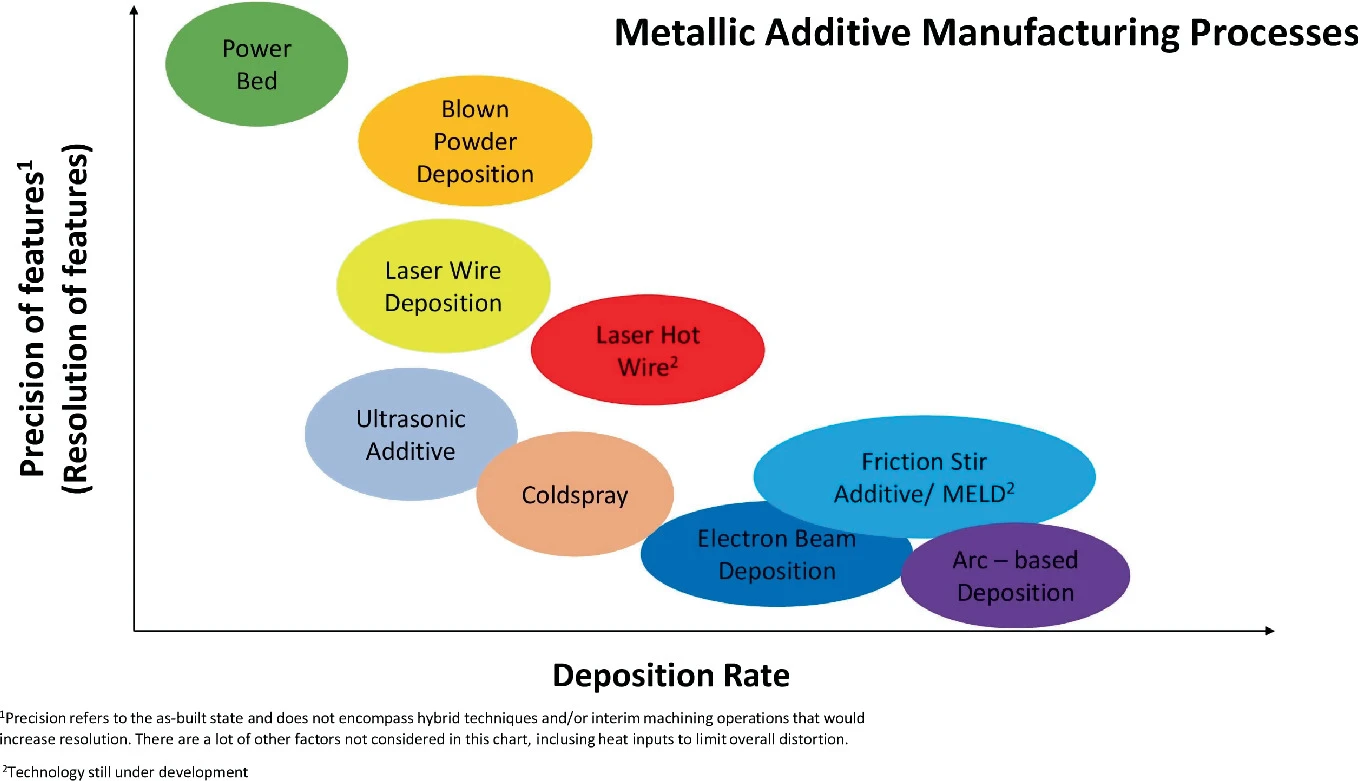
\includegraphics[width=\textwidth]{../report_assets/am-comparrison.png}
        \caption{Current feed system diagram\cite{Ramoni2022}.}\label{fig:am-methods-comparison}
    \end{minipage}

\end{figure}

Friction Stir Deposition (FSD) is a process that uses a rotating tool to create frictional heat and plastic deformation in the material, allowing it to be deposited onto a substrate. This process has a high deposition rate, but the need for a rotating tool, changover of this tool and the low technology readiness level (TRL) of 4\cite{nasa2025fsd} excludes it from benefiting much from research into its space applications at this stage.
Arc-based deposition methods, such as Wire Arc Additive Manufacturing (WAAM) have already been investigated for in-space applications and show great promise. However, these direct energy deposition (DED) methods are not suitable for all manufacturing applications due to melting the material, which can lead to residual stresses and distortion in the final part\cite{PATTISON2007627}. Laser Hot Wire and Electron Beam Melting also fall into this category but one could argue they are even less suitable due to geometry restrictions and additional system complexity respectively.


maybe talk about sls and other powder bed stuff


This leaves a gap in current research for a high deposition rate, non-thermal additive manufacturing process that is suitable for in-space applications. Cold Spray Additive Manufacturing (CSAM) is a promising candidate to fill this gap, as it has a high deposition rate, a wide range of materials available, and is non-thermal in nature. 

\section{Cold Spray}
CSAM works by accelerating metal powder particles to supersonic speeds using high velocity gas, causing them to deform and bond to a substrate. 

Any atomically-flat clean surfaces of metal will bond together when they come into contact in a vacuum\cite{holzbauer2024}. This is known as cold welding and works because the surface energy of the metals seperated is higher than that of them bonded together and so they move towards the lower energy state. The atoms undergo surface diffusion and rearrangement along their crystaline structures\cite{ctx46070057700001591} to form this metallic bond. 

While the particles themselves are often coated in an oxide layer, the high velocity of the impact causes the oxide layer to be removed, exposing the clean metal surface underneath. This is thought to be caused by adiabatic shear instability at the interface that breaks up the layer\cite{assadi2016cold}. This is a key feature of cold spray, as it allows for the bonding of materials that would otherwise be difficult to weld or bond together.


While it is debated in literature the exact nature of this deformation ...
As the particle impacts the substrate, it undergoes compaction into the substrate as well as metallurgically bonding over a significant portion of the contact area.
\subsection{Core Process}
When a particle is accelerated to a high velocity, it undergoes plastic deformation upon impact with the substrate. This deformation causes the particles to bond together, creating a solid layer of material. 

key parameters
\subsection{Advantages}
compare to other am techniques
\subsection{Space Applications}

gaps in research

\section{COSMOS}
aims, objectives, results and limitations








rejig after 5 page review

\section{Space as Resource}
Space plays a vital role in advancing science, technology, and the broader progress of humanity. Through the exploration of space, scientists gain unique insights into the origins of the universe, the behavior of physical laws under extreme conditions, and the potential for life elsewhere in the universe. Along with scientific descoveries, technological developments driven by space research often find critical applications on Earth. From satellite television to microwaves, space technology improves everyday life and drives innovation across industries. Beyond tangible benefits, space exploration fosters curiosity, unity, and ambition, encouraging humanity to transcend borders and collaborate on solving challenges that face us collectively. As we expand our presence outside Earth, space becomes not only a frontier of discovery but also a catalyst for technological and social progress on a global scale.

\section{Space as a Manufacturing Environment}
In-space manufacturing is currently experiencing a surge in interest due to the decreasing cost per kilogram of putting payloads into orbit. With the expectation that Starship will soon reduce this price from around \$1000/kg to \$150/kg~\cite{nextbigfuture2024spacex}, there will be a plethora of new opportunities available to those that can successfully leverage this exotic environment. Microgravity, high vacuum and abundant solar energy are all inherent to space, while remaining very expensive to achieve on Earth. Therefore, products that can utilise these during the manufacturing process would be more cost competitive or higher quality than those made on the ground.

In many state-of-the-art materials, fabrication under microgravity results in bigger crystal growth and a more homogenous structure~\cite{issnll_mccg}. This is hugely beneficial for superconducting applications as they are constrained by the inability to sustain high currents, a limitation caused by the presence of grain boundaries~\cite{hilgenkamp2002grain}. Superconductors are, therefore, a perfect candidate for in-space manufacturing and higher quality crystals could unlock new terrestrial applications.

In the longer term, an industrial base in low earth orbit would also have significant implications for the future of space. Violent launch conditions that the spacecraft's structure must withstand before reaching orbit places a harsh design constraint on all current missions. Manufacturing or assembling key components in space would circumvent this, increasing mission flexibility and reliability. At present, solar sail technology is limited by payload fairing dimensions and must be able to fold down to fit within these. If the frames were manufactured in orbit, it would massively decrease mission complexity, enabling new propulsion platforms.

\newpage
\section{Additive Manufacturing in Space CLEAN}
Additive manufacturing, also known as 3D printing, is a transformative technology that enables the layer-by-layer construction of complex structures from stock material. This approach is particularly well suited to space manufacturing due to its low material waste, high design flexibility, and the ease of transporting feedstock like filament or powder. Prefabricated components like I-beams or plates struggle to efficiently pack into launch vehicle payload fairings if large dimensions are required. In comparison, raw materials for additive manufacturing can be stored in any geometry and are adaptable to a wide range of mission needs.

For structural components of any space mission, the requirements to be compact enough to fit into the payload fairing and strong enough to withstand the launch vibrations sacrifice [efficiency and reliability wantt o get across big optimisation problem]. If these parts are manufactured once they are in orbit, the designs can be tailored to the orbital manoeuvre loads alone, increasing mission flexibility.!!

Additionally!!, the crucial benefit of additive manufacturing is its ability to repair and modify existing components. This capability is especially valuable in space, where repairs can!! be challenging and costly. By enabling on-demand production of spare parts or modifications to existing systems, additive manufacturing enhances the resilience and longevity of space missions, reducing the need for extensive inventories of spare parts and minimizing the risk of mission failure due to component obsolescence or damage.!!



\section{Objectives}
As mentioned, the previous powder hopper design of the COSMOS project, seen in \autoref{fig:current-feed-system-exploded-diagram}, was not suitable for microgravity applications. It resembles a typical fluidized powder bed used in the chemical engineering industry, seen in \autoref{fig:fluidized-bed-diagram}, where the gas flows from bottom to top and, given a high enough flow rate, entrains the particles into the flow.
\begin{figure}[htbp]
    \centering

    \begin{minipage}{0.3\textwidth}
        \centering
        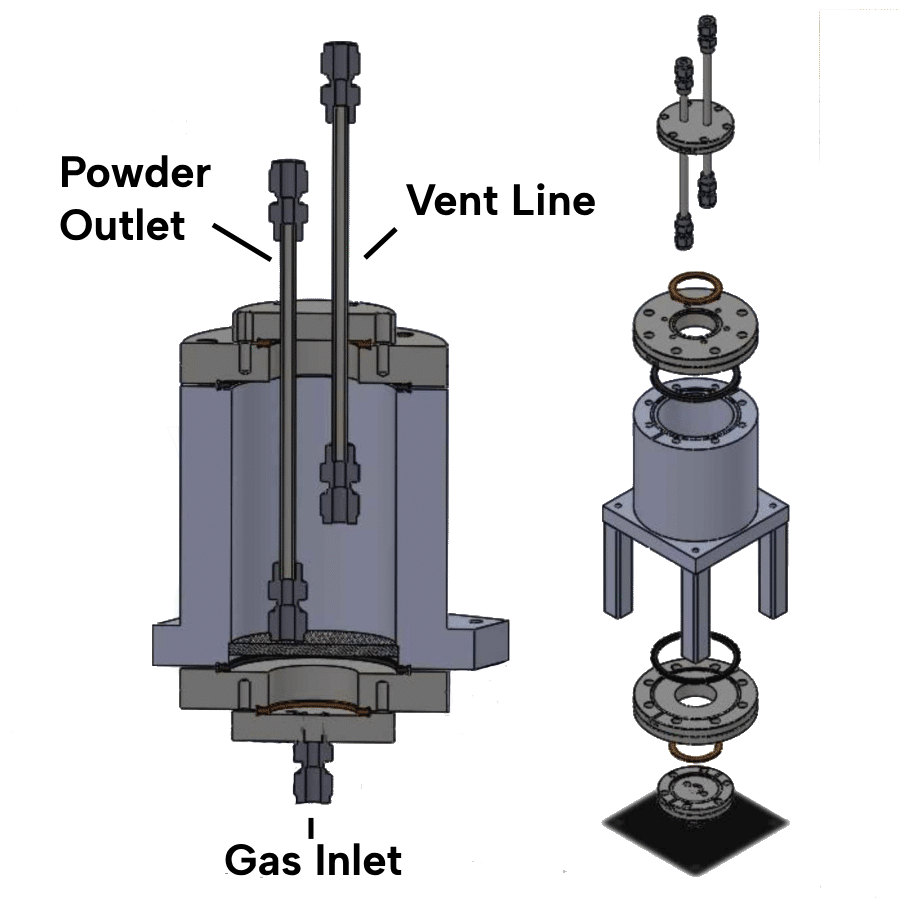
\includegraphics[width=\textwidth]{../report_assets/COSMOS_DIAGRAM.png}
        \caption{Current feed system diagram.}\label{fig:current-feed-system-exploded-diagram}
    \end{minipage}
    \hfill
    \begin{minipage}{0.3\textwidth}
        \centering
        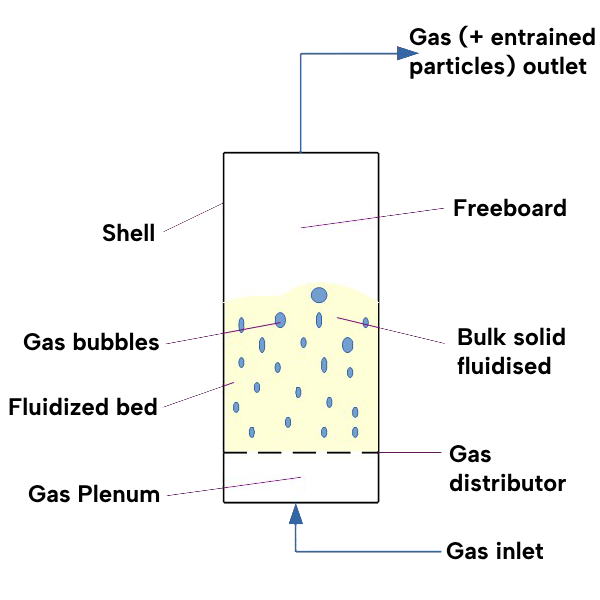
\includegraphics[width=\textwidth]{../report_assets/Fluidized_Bed_polished.png}
        \caption{Simplified fluidized powder bed diagram.}\label{fig:fluidized-bed-diagram}
    \end{minipage}
    \hfill
    \begin{minipage}{0.3\textwidth}
        \centering
        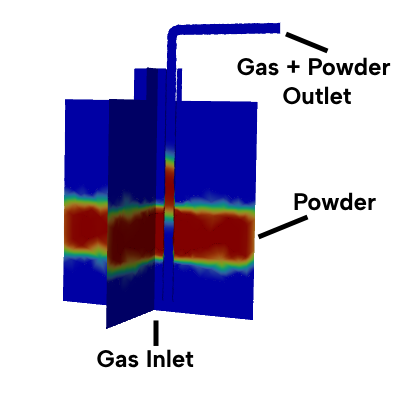
\includegraphics[width=\textwidth]{../report_assets/configuration_that_demands_pms.png}
        \caption{Fluent simulation in microgravity.}\label{fig:current-feed-system-fluent}
    \end{minipage}

\end{figure}

While it was more than suitable to facilitate the testing of the CSAM system, in a space environment, it would be prone to disruption due to the powder drifting away from the outlet. This is because the powder, that sat on top of the mesh in the experiments, is not constrained to this location by anything but gravity. Therefore, if the tank were to recieve a sloshing perturbance, the powder would float off the mesh and away from the outlet. To verify this idea and demonstrate that the powder would not be dispersed throughout the whole tank due to turbulent mixing, a fluent simulation was conducted, seen in \autoref{fig:current-feed-system-fluent}. Even after 10s of simulation time the system reached steady state with no mixing or powder dispersion, necesitating a redesign.

Building on all this previous work, the primary objectives of the project were to develop and characterise a tank capable of producing a constant and controllable mass flow rate as well as operating reliably under microgravity. The tank must:
\begin{itemize}
    \item Constrain the powder to the outlet of the system in microgravity,
    \item Design for controlability of the mass flow rate,
    \item Resist pressurisation and depresurisation faults.
\end{itemize}
And to characterise this system, the relationship between pressure into the system and mass flow rate out must be defined through:
\begin{itemize}
    \item Analysing the relationship between piston velocity and mass flow rate,
    \item Analysing the relationship between pressure differentials across the piston face and the corresponding velocity,
    \item Determine key factors in piston geometry that affect the pressure differential.
\end{itemize}


\subsection{Hopper tank design}
As seen in \autoref{appendix:feed-architecture-analysis}, there are many ways the feed system can be messed up, especially around pressurising and depressurising the vessle. Therefore, for the tank to perform its function correctly, it must be resistant to these problems as well as managing the position of the powder during operations. Typically, fluid containing tanks can use the plethora of propellant management devices which take advantage of surface tension to keep the fuel close to the outlet. For this tank, this isn't possible and so a piston design was used. This has the advantage of being another component of the system that can be optimised to achieve the desired mass flow rate but has implications for the rest of the design. The piston is much better suited to long thin tank designs which typically perform worse under high pressures than their circular counterparts. Additionally, the demands on the geometry make it harder to scale up. The aspect ratio of the piston is important to prevent cocking!!!cite!!! so a wider tank requires a much bigger piston and a longer tank may have implications on the inlet pressure required due to the flow through the powder reducing the static pressure of the gas!!!check this is true!!!



\subsection{Choke Point}
It is proposed that the flow characteristics of the fluidised powder bed system are simpler, therefore easier to control, if the flow is choked.!!validate this as not in design anymore!!


This chokepoint then needs to withstand getting sand blasted as to not change the throat area over time. The most ideal solution to this problem involves very hard materials like!!! or!!! that can withstand the powder for many tests. Given the scope of this project, however, one-time use 3D printed chokepoints were used. They were made of PLA which has a hardness of~!!! and is expected to wear away at a rate of~!!!. This was deemed experimentally acceptable because of a change in throat diameter of~!!! over~!!! doesnt significantly alter the results.
